% =============================================================================
% APENDICE C: VISUALIZACIONES ADICIONALES
% =============================================================================

\chapter{Visualizaciones Adicionales}
\label{ap:visualizaciones}

Este apendice recopila las visualizaciones generadas durante el desarrollo del proyecto, organizadas por categoria.

% -----------------------------------------------------------------------------
\section{Diagramas de Arquitectura}
\label{sec:ap_diagramas}
% -----------------------------------------------------------------------------

Los diagramas de arquitectura se encuentran en el directorio \texttt{outputs/diagrams/}:

\begin{table}[htbp]
    \centering
    \caption{Diagramas de arquitectura generados}
    \label{tab:ap_diagrams}
    \begin{tabular}{@{}lp{8cm}@{}}
        \toprule
        \textbf{Archivo} & \textbf{Descripcion} \\
        \midrule
        model\_architecture.png & Diagrama de bloques del modelo completo \\
        coordinate\_attention.png & Detalle del modulo CoordinateAttention \\
        ensemble\_tta\_pipeline.png & Pipeline de inferencia con ensemble + TTA \\
        training\_pipeline.png & Diagrama del entrenamiento en 2 fases \\
        data\_flow.png & Flujo de datos simplificado \\
        \bottomrule
    \end{tabular}
\end{table}

\begin{figure}[htbp]
    \centering
    \includegraphics[width=\textwidth]{model_architecture.png}
    \caption{Arquitectura completa del modelo. La imagen de entrada pasa por ResNet-18, Coordinate Attention, Global Average Pooling y la cabeza de regresion profunda.}
    \label{fig:ap_architecture}
\end{figure}

\begin{figure}[htbp]
    \centering
    \includegraphics[width=\textwidth]{training_pipeline.png}
    \caption{Pipeline de entrenamiento en dos fases. Fase 1: backbone congelado (15 epocas). Fase 2: fine-tuning completo (100 epocas).}
    \label{fig:ap_training}
\end{figure}

\begin{figure}[htbp]
    \centering
    \includegraphics[width=\textwidth]{ensemble_tta_pipeline.png}
    \caption{Pipeline de inferencia con ensemble y TTA. Cada imagen genera 8 predicciones (4 modelos $\times$ 2 augmentaciones) que se promedian.}
    \label{fig:ap_ensemble}
\end{figure}

% -----------------------------------------------------------------------------
\section{Figuras de Resultados}
\label{sec:ap_resultados}
% -----------------------------------------------------------------------------

Las figuras de resultados se encuentran en el directorio \texttt{outputs/thesis\_figures/}:

\begin{table}[htbp]
    \centering
    \caption{Figuras de resultados generadas}
    \label{tab:ap_figures}
    \begin{tabular}{@{}lp{8cm}@{}}
        \toprule
        \textbf{Archivo} & \textbf{Descripcion} \\
        \midrule
        progress\_by\_session.png & Evolucion del error por sesion \\
        error\_by\_landmark.png & Error por landmark (15 barras) \\
        error\_by\_category.png & Comparacion por categoria \\
        heatmap\_landmark\_category.png & Heatmap de errores \\
        ensemble\_comparison.png & Modelos individuales vs ensemble \\
        ablation\_study.png & Contribucion de cada mejora \\
        summary\_table.png & Tabla resumen del proyecto \\
        clahe\_comparison.png & Efecto de CLAHE \\
        prediction\_examples.png & Ejemplos de predicciones \\
        best\_worst\_cases.png & Mejores y peores casos \\
        \bottomrule
    \end{tabular}
\end{table}

\begin{figure}[htbp]
    \centering
    \includegraphics[width=0.9\textwidth]{progress_by_session.png}
    \caption{Progreso del error a lo largo de las 15 sesiones de desarrollo. La linea muestra la reduccion progresiva desde 9.08 px (baseline) hasta 3.71 px (ensemble final).}
    \label{fig:ap_progress}
\end{figure}

\begin{figure}[htbp]
    \centering
    \includegraphics[width=0.9\textwidth]{ablation_study.png}
    \caption{Estudio de ablacion: contribucion de cada componente. El ensemble y CLAHE son los que mayor impacto tienen en la reduccion del error.}
    \label{fig:ap_ablation}
\end{figure}

% -----------------------------------------------------------------------------
\section{Visualizacion de Predicciones}
\label{sec:ap_predicciones}
% -----------------------------------------------------------------------------

\begin{figure}[htbp]
    \centering
    \includegraphics[width=\textwidth]{prediction_examples.png}
    \caption{Ejemplos de predicciones del ensemble en las tres categorias diagnosticas. Circulos verdes: ground truth; Cruces rojas: prediccion del modelo. Se observa alta precision en los tres tipos de imagenes.}
    \label{fig:ap_examples}
\end{figure}

\begin{figure}[htbp]
    \centering
    \includegraphics[width=\textwidth]{best_worst_cases.png}
    \caption{Mejores y peores casos del conjunto de prueba. Arriba: casos con menor error ($<$ 2 px promedio). Abajo: casos con mayor error ($>$ 8 px promedio). Los peores casos corresponden a imagenes con patologia severa o artefactos.}
    \label{fig:ap_best_worst}
\end{figure}

% -----------------------------------------------------------------------------
\section{Comparacion CLAHE}
\label{sec:ap_clahe}
% -----------------------------------------------------------------------------

\begin{figure}[htbp]
    \centering
    \includegraphics[width=\textwidth]{clahe_comparison.png}
    \caption{Efecto visual de CLAHE en radiografias de las tres categorias. Izquierda: imagen original. Derecha: imagen con CLAHE (clip=2.0, tile=4). Se observa mejor definicion de bordes anatomicos, especialmente en las consolidaciones de COVID-19.}
    \label{fig:ap_clahe}
\end{figure}

% -----------------------------------------------------------------------------
\section{Anatomia de Landmarks}
\label{sec:ap_anatomia}
% -----------------------------------------------------------------------------

\begin{figure}[htbp]
    \centering
    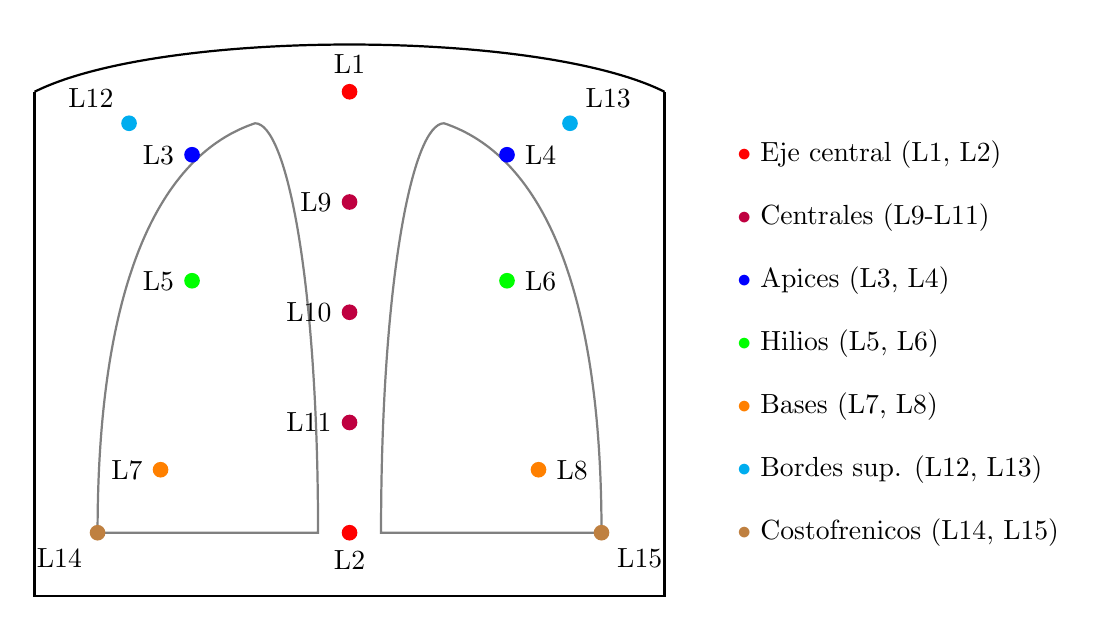
\begin{tikzpicture}[scale=0.8]
        % Silueta de torax simplificada
        \draw[thick] (0,8) -- (0,0) -- (10,0) -- (10,8);
        \draw[thick] (0,8) .. controls (2,9) and (8,9) .. (10,8);

        % Pulmones (simplificados)
        \draw[gray, thick] (1,1) .. controls (1,5) and (2,7) .. (3.5,7.5)
                          .. controls (4,7.5) and (4.5,5) .. (4.5,1) -- cycle;
        \draw[gray, thick] (9,1) .. controls (9,5) and (8,7) .. (6.5,7.5)
                          .. controls (6,7.5) and (5.5,5) .. (5.5,1) -- cycle;

        % Landmarks con etiquetas
        \node[circle, fill=red, inner sep=2pt, label=above:L1] at (5,8) {};
        \node[circle, fill=red, inner sep=2pt, label=below:L2] at (5,1) {};

        \node[circle, fill=blue, inner sep=2pt, label=left:L3] at (2.5,7) {};
        \node[circle, fill=blue, inner sep=2pt, label=right:L4] at (7.5,7) {};

        \node[circle, fill=green, inner sep=2pt, label=left:L5] at (2.5,5) {};
        \node[circle, fill=green, inner sep=2pt, label=right:L6] at (7.5,5) {};

        \node[circle, fill=orange, inner sep=2pt, label=left:L7] at (2,2) {};
        \node[circle, fill=orange, inner sep=2pt, label=right:L8] at (8,2) {};

        \node[circle, fill=purple, inner sep=2pt, label=left:L9] at (5,6.25) {};
        \node[circle, fill=purple, inner sep=2pt, label=left:L10] at (5,4.5) {};
        \node[circle, fill=purple, inner sep=2pt, label=left:L11] at (5,2.75) {};

        \node[circle, fill=cyan, inner sep=2pt, label=above left:L12] at (1.5,7.5) {};
        \node[circle, fill=cyan, inner sep=2pt, label=above right:L13] at (8.5,7.5) {};

        \node[circle, fill=brown, inner sep=2pt, label=below left:L14] at (1,1) {};
        \node[circle, fill=brown, inner sep=2pt, label=below right:L15] at (9,1) {};

        % Leyenda
        \node[anchor=west] at (11, 7) {\textcolor{red}{$\bullet$} Eje central (L1, L2)};
        \node[anchor=west] at (11, 6) {\textcolor{purple}{$\bullet$} Centrales (L9-L11)};
        \node[anchor=west] at (11, 5) {\textcolor{blue}{$\bullet$} Apices (L3, L4)};
        \node[anchor=west] at (11, 4) {\textcolor{green}{$\bullet$} Hilios (L5, L6)};
        \node[anchor=west] at (11, 3) {\textcolor{orange}{$\bullet$} Bases (L7, L8)};
        \node[anchor=west] at (11, 2) {\textcolor{cyan}{$\bullet$} Bordes sup. (L12, L13)};
        \node[anchor=west] at (11, 1) {\textcolor{brown}{$\bullet$} Costofrenicos (L14, L15)};
    \end{tikzpicture}
    \caption{Diagrama esquematico de la ubicacion de los 15 landmarks anatomicos en una radiografia de torax. Los landmarks centrales (L9, L10, L11) dividen el eje L1-L2 en proporciones de 0.25, 0.50 y 0.75.}
    \label{fig:ap_landmarks}
\end{figure}

% -----------------------------------------------------------------------------
\section{Scripts de Generacion}
\label{sec:ap_scripts}
% -----------------------------------------------------------------------------

Los scripts utilizados para generar las visualizaciones se encuentran en \texttt{scripts/visualization/}:

\begin{table}[htbp]
    \centering
    \caption{Scripts de visualizacion}
    \label{tab:ap_scripts}
    \begin{tabular}{@{}lp{8cm}@{}}
        \toprule
        \textbf{Script} & \textbf{Descripcion} \\
        \midrule
        generate\_architecture\_diagrams.py & Genera diagramas de arquitectura usando matplotlib \\
        generate\_results\_figures.py & Genera graficos de resultados y tablas \\
        generate\_prediction\_samples.py & Genera visualizaciones de predicciones \\
        \bottomrule
    \end{tabular}
\end{table}

\begin{lstlisting}[caption={Ejemplo de uso de scripts de visualizacion},label={lst:ap_vis_usage},language=bash]
# Generar todos los diagramas de arquitectura
python scripts/visualization/generate_architecture_diagrams.py \
    --output-dir outputs/diagrams/

# Generar figuras de resultados
python scripts/visualization/generate_results_figures.py \
    --results-file outputs/evaluation_results.json \
    --output-dir outputs/thesis_figures/

# Generar ejemplos de predicciones
python scripts/visualization/generate_prediction_samples.py \
    --checkpoint checkpoints/ensemble/ \
    --num-samples 10 \
    --output-dir outputs/thesis_figures/
\end{lstlisting}

% -----------------------------------------------------------------------------
% FIN DEL APENDICE
% -----------------------------------------------------------------------------
